\section{Introduction}
\label{sec:introduction}

\begin{figure}[b]
\centering
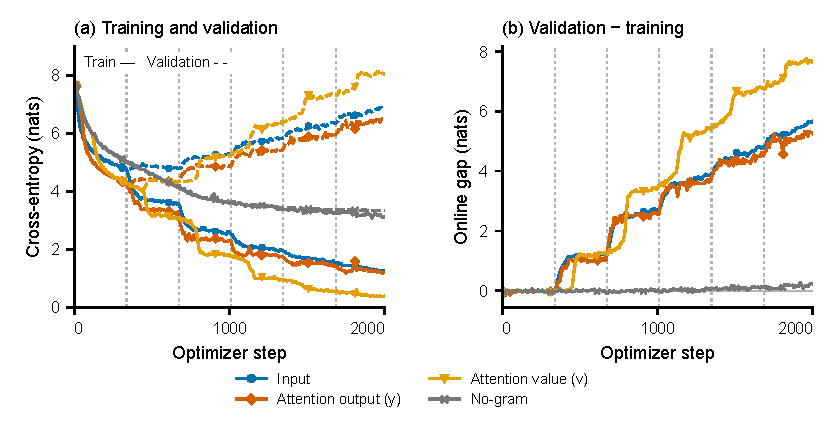
\includegraphics[width=\linewidth]{fig01_forking.pdf}
\caption{Forking under fixed data replay.}
\label{fig:injection-curves}
\end{figure}


Language-model agents are increasingly used to propose, execute, and evaluate research ideas. Systems for automated scientific discovery and model improvement extend this process from individual coding tasks to iterative experimental search \citep{lu2024scientist,recursive2026research}. Such searches can improve a target metric, but they can also reveal behavior that was not part of the original objective. This paper studies one such discovery in a NanoGPT autoresearch workflow.

The agent's task was to modify the model architecture and trainer to minimize next-token validation bits per byte (BPB). During a small-data experiment, we observed an unexpected pattern: Training and validation losses initially improved together, But once the loader began replaying previously seen text, the curves separated rapidly near the epoch boundary. Training loss continued to fall, while validation loss stopped improving or even increased. The gap then grew in steps over subsequent passes. We call this replay-aligned divergence \emph{forking} (Figure~\ref{fig:injection-curves}).

This behavior resembles overfitting: training loss continues to decrease while validation loss deteriorates, a pattern previously observed in language models trained on repeated data \citep{hernandez2022repeated}. However, such a sharp divergence is not an inevitable consequence of data reuse; previous studies show that language models can benefit from several passes over a finite corpus \citep{muennighoff2023scaling}. Through a series of controlled experiments, we trace forking to the interaction between data replay and \emph{over-encoding}, which enriches token representations with additional embeddings of local token combinations \citep{huang2025over}. In our model, an $n$-gram module uses the most recent $n$ tokens, including the current token, to retrieve a learned embedding from a hash-indexed table. This embedding is injected into the Transformer backbone to help predict the next token. Across the configurations we test, adding this module produces a pronounced training--validation gap once the training data are replayed.

To understand why over-encoding promotes overfitting under replay, we examine how the gap depends on context frequency. Low-frequency $n$-gram contexts account for a substantial share of the additional gap, and the average gap follows an approximate power-law relationship with context frequency over the measured range. We propose that the $n$-gram table makes optimization more local by assigning distinct learned representations to different contexts. These representations allow the model to fit local prediction problems more independently, making it easier to memorize the continuations observed in training. For rare contexts, only a few valid continuations may be represented in the corpus. Replaying the same examples reinforces these continuations without expanding their coverage, potentially suppressing alternatives needed at validation time. We develop this explanation through frequency-dependent interventions, a model of continuation coverage, and an analysis of replay dynamics.

